\namedchapter{Konstrukcja mechaniczna}
\namedsection[Adam Zieliński]{Model 3D}
Proces budowy robota rozpoczął się od stworzenia trójwymiarowego modelu pojazdu. Projekt wykonany został przy wykorzystaniu studenckiej wersji oprogramowania Autodesk Inventor Professional 2014. Symulacja 3D miała na celu przede wszystkim ukazanie złożoności całego projektu. Pozwoliła m.in. na dokładne rozmieszczenie wszystkich komponentów wraz z uwzględnionymi rzeczywistymi wymiarami. Na rysunku \ref{mod3d} przedstawiony został uzyskany efekt wraz z naniesionymi oznaczeniami poszczególnych elementów. 

  \begin{figure}[H]
    \begin{center}
      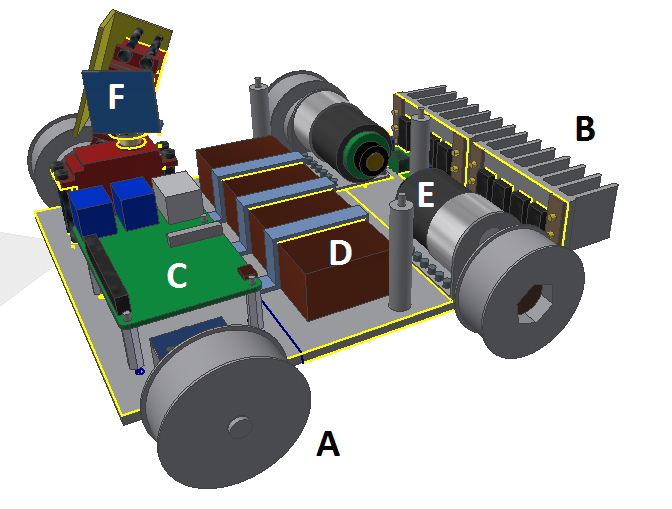
\includegraphics[scale=0.55]{imgs/calosc_2.png}
 	\caption[Model 3D projektowanego czołgu.]{\small{Model 3D projektowanego pojazdu. A - koła, B - mostki H wraz z radiatorami, C - Raspberry 2 Pi Model B, D - bateria, E - silniki prądu stałego, F - wieżyczka}}
	\label{mod3d}
    \end{center}
  \end{figure}
\namedsection[Adam Zieliński]{Podstawa pojazdu}
Wszystkie elementy zgrupowane na rysunku \ref{mod3d} tworzą korpus pojazdu, który został osadzony na sklejce brzozowej o grubości 5 mm. Materiał został wybrany pod kątem łatwości w obróbce oraz trwałości. Ze względu na jego warstwową strukturę jest on bardzo wytrzymały i jednocześnie bardzo lekki. Wyżej omówiony model 3D pozwolił jednoznacznie dobrać wymiary podstawy oraz bardzo dokładnie wskazać miejsca, w których należało wykonać otwory mocujące dla poszczególnych komponentów. 

  \begin{figure}[H]
    \begin{center}
      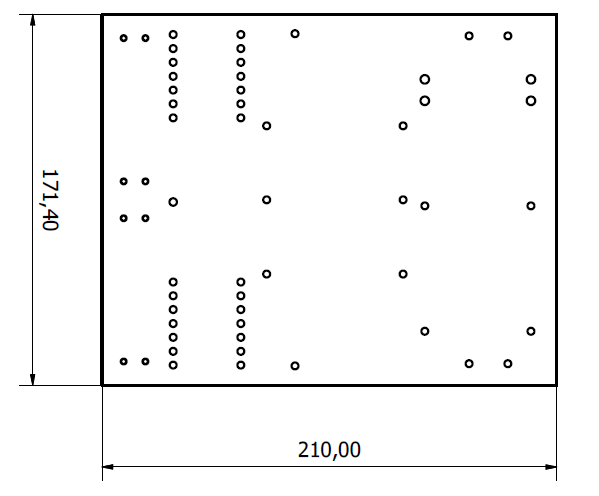
\includegraphics[scale=0.55]{imgs/podstawa.png}
 	\caption[Podstawa pojazdu.]{\small{Podstawa pojazdu wraz z naniesionymi wymiarami w milimetrach i otworami niezbędnymi do zamocowania poszczególnych elementów.}}
	\label{podst3d}
    \end{center}
  \end{figure}
\namedsection[Adam Zieliński]{Wieżyczka}
Wieża pojazdu zbudowana została w oparciu o 2 serwa modelarskie TowerPro SG-5010. Serwomechanizmy są zintegrowanymi układami elektronicznymi zawierającymi sekcję mechaniczną - silnik, oraz układ sterowania położeniem.
Na rysunku \ref{wieza3d} przedstawiono model omawianego segmentu. Serwo A jest zamocowane bezpośrednio do podstawy pojazdu i dzięki niemu realizowany jest obrót prawo/lewo wieży. Do orczyka, czyli obrotowej części mechanizmu, zamocowane zostało mocowanie drugiego serwa(B). Wykonane zostało ono z aluminiowego kątownika. Aluminium bardzo dobrze nadaje się do tego typu rozwiązań ponieważ jest tanie, łatwo dostępne, lekkie i stosunkowo wytrzymałe.  

  \begin{figure}[H]
    \begin{center}
      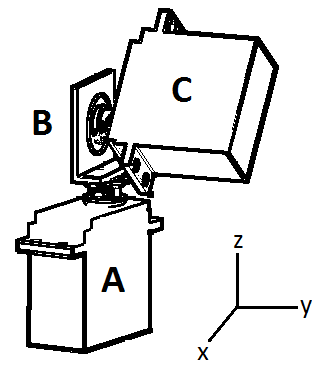
\includegraphics[scale=0.45]{imgs/wieza_3d.png}
 	\caption[Model wieżyczki.]{\small{Trójwymiarowy model konstrukcji wieżyczki czołgu. A - serwomechanizm odpowiedzialny za obrót wokół osi OZ, B - serwomechanizm obrotu w osi OY, C - łączenie pomiędzy elementami.}}
	\label{wieza3d}
    \end{center}
  \end{figure}
\namedsection[Adam Zieliński]{Napęd}
Robot mobilny powinien móc swobodnie poruszać się w środowisku w jakim się znajduje. Wymusza to wykorzystanie możliwie wydajnych napędów o niewielkich gabarytach. W projekcie wykorzystano dwa szczotkowe silniki prądu stałego Pololu 37Dx52L wraz z przekładnią 30:1. Dla napięcia 12 woltów pojedynczy silnik moment obrotowy wynoszący 8 kg$\cdot$cm i obracają się z prędkością 350 obrotów na minutę. Rysunek techniczny przedstawiający dokładne wymiary wykorzystanego silnika przedstawiono na rysunku \ref{wymiary_silnika}. Maksymalny pobór prądu (przy zatrzymaniu wału) może wynieść około 5 A.

  \begin{figure}[H]
    \begin{center}
      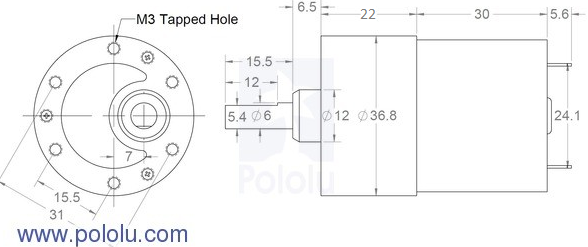
\includegraphics[scale=0.7]{imgs/silnik_wymiary.png}
 	\caption[Wymiary silnika Pololu 37Dx52L ]{\small{Wymiary wykorzystane silnika - Pololu 37Dx52L }\footnotemark}
	\label{wymiary_silnika}
    \end{center}
  \end{figure}
  \footnotetext{http://pololu.com/, (data dostępu 20.10.2015r.)}

Jednym z założeń początkowych było zastosowanie w pojeździe napędu gąsienicowego. Był to dość trudny do rozwiązania problem ze względu na brak specjalizowanych rozwiązań w tym kierunku. Dodatkowo sprawę komplikują nietypowe wymiary pojazdu. Od początku zakładaliśmy, że cały robot nie będzie zbudowany pod pewien konkretny rozstaw kół, ale gąsienice dobrane będą na podstawie uzyskanych wymiarów. Ostatecznie robot zbudowany został w oparciu o 4 koła metryczne 27T5/32. Są to wykonane z aluminium koła pasowe stosowane w przemyśle do przełożenia napędu. Ich średnica to 54 mm. Razem z dedykowanym pasem zębatym T5 o długości 420 mm tworzą układ gąsienic. Na ilustracji \ref{gasienice_elementy} przedstawione zostały wykorzystane elementy.

  \begin{figure}[H]
    \begin{center}
      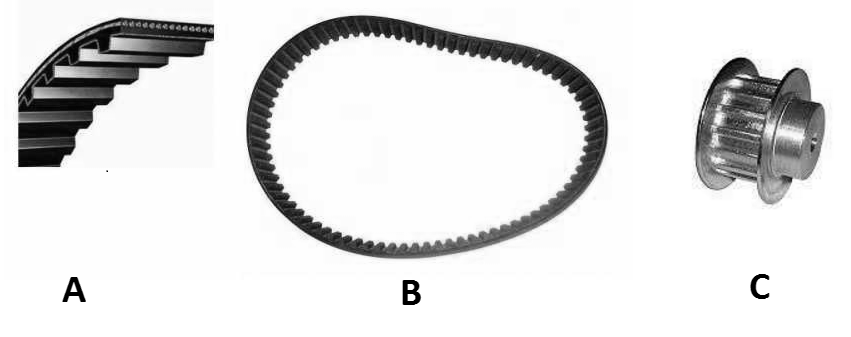
\includegraphics[scale=0.5]{imgs/gasienice.png}
 	\caption[Elementy gąsienic.]{\small{Rysunki A i B przedstawiają pas zębaty T5, C - koło zębate T5. }\footnotemark}
	\label{gasienice_elementy}
    \end{center}
  \end{figure}
  \footnotetext{http://centrum-cnc.pl/, (data dostępu 29.10.2015r.)}

Wybrane przez nas koła metryczne posiadały na środku otwór o średnicy 8 mm, podczas gdy oś silników ma średnicę 6 mm. Należało zatem wykonać mocowanie, pozwalające na sztywne osadzenie kół na wale napędowym. Do tego celu wykorzystaliśmy otrzymane wraz z silnikami sześciokątne nakładki, przedstawione na rysunku \ref{zamocowanie_szesciokatne}. Wycięcie w aluminium otworu w kształcie sześciokąta w warunkach domowych jest bardzo trudne. W związku z czym, dzięki projektowi w środowisku CAD, możliwe było zlecenie wykonania go firmie zewnętrznej, specjalizującej się w cięciu wodą pod wysokim ciśnieniem.

  \begin{figure}[H]
    \begin{center}
      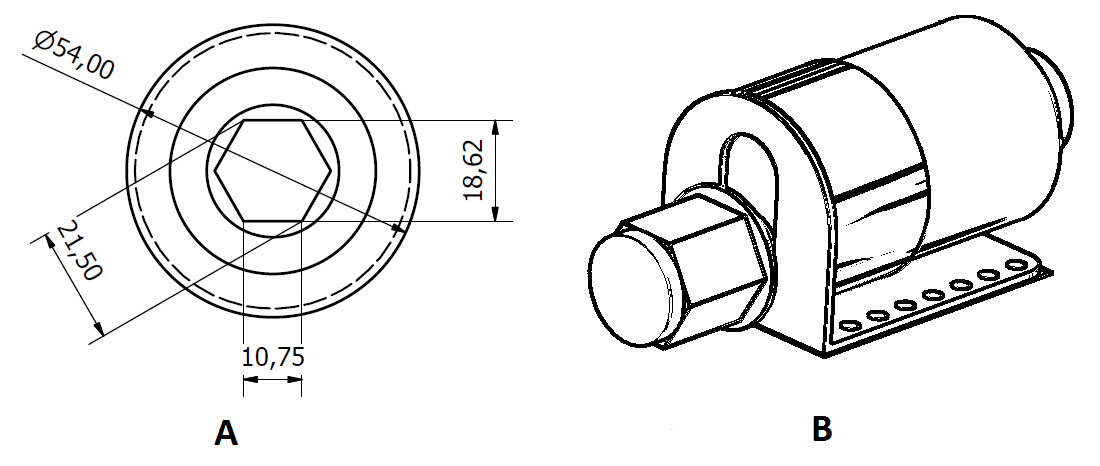
\includegraphics[scale=0.40]{imgs/moc_kol_tyl.png}
 	\caption[Model tylnych kół.]{\small{Na ilustracji znajduje się rysunek techniczny koła metrycznego(A) dostosowanego na potrzeby mocowania na silniku z wykorzystaniem sześciokątnej przejściówki(B).}}
	\label{zamocowanie_szesciokatne}
    \end{center}
  \end{figure}

Należało także rozważyć projekt mocowania przednich kół. Ze względu na fakt, iż gąsienice (prawa/lewa) mogą obracać się jednocześnie w dwóch rożnych kierunkach należało zastosować osobną oś dla prawego oraz lewego koła. Jej model przedstawiony został na rysunku \ref{zamocowanie_przod}. Element A wykonany został z drewna dębowego, które jest mało elastyczne - co pozwala na dokładne spasowanie z osią, zaznaczoną listerą B, która wykonana została na tokarni z aluminium.

  \begin{figure}[H]
    \begin{center}
      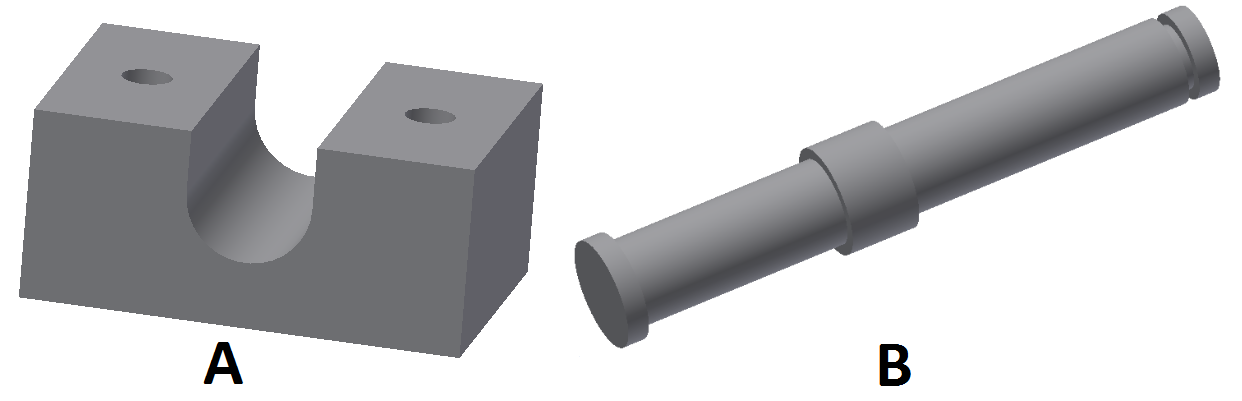
\includegraphics[scale=0.40]{imgs/moc_kol_prz.png}
 	\caption[Model mocowania kół przednich.]{\small{Na rysunku przedstawiony został model wykonania mocowań kół przednich pojazdu. A - przedstawia blok łączący oś (B) z podstawą czołgu.}}
	\label{zamocowanie_przod}
    \end{center}
  \end{figure}